%%%%%%%%%%%%%%%%%%%%%%%%%%%%%%%%%%%%%%%%%%%%%%%%%%%%%%%%%%%%%%%%%%%%%%%
%%%%%%%%%%%%%%%%%%%%%%%%%%%%%%%%%%%%%%%%%%%%%%%%%%%%%%%%%%%%%%%%%%%%%%%
%%%%%                                                                 %
%%%%%     Carl_Friess_BachelorThesis.tex                              %
%%%%%                                                                 %
%%%%% Author:      Carl Friess                                        %
%%%%% Created:     21-Aug-2018                                        %
%%%%% Description: BachelorThesis                                     %
%%%%%                                                                 %
%%%%%%%%%%%%%%%%%%%%%%%%%%%%%%%%%%%%%%%%%%%%%%%%%%%%%%%%%%%%%%%%%%%%%%%
%%%%%%%%%%%%%%%%%%%%%%%%%%%%%%%%%%%%%%%%%%%%%%%%%%%%%%%%%%%%%%%%%%%%%%%

%%%%%%%%%%%%%%%%%%%%%%%%%%%%%%%%%%%%%%%%%%%%%%%%%%%%%%%%%%%%%%%%%%%%%%%
%%%%%                                                                 %
%%%%%     Document Class                                              %
%%%%%                                                                 %
%%%%%%%%%%%%%%%%%%%%%%%%%%%%%%%%%%%%%%%%%%%%%%%%%%%%%%%%%%%%%%%%%%%%%%%
\documentclass[%
 oneside,      % Use the same margins for odd and even pages (cannot
               % be used with the 'twoside' option). 
% twoside,      % Use different margins for odd and even pages (cannot
               % be used with the 'oneside' option).
 openany,      % Open chapters on odd and even pages.
 halfparskip,  % Create small spaces for new paragraphs but no indents.
]{scrbook}

%%%%%%%%%%%%%%%%%%%%%%%%%%%%%%%%%%%%%%%%%%%%%%%%%%%%%%%%%%%%%%%%%%%%%%%
%%%%%                                                                 %
%%%%%     Preamble                                                    %
%%%%%                                                                 %
%%%%%%%%%%%%%%%%%%%%%%%%%%%%%%%%%%%%%%%%%%%%%%%%%%%%%%%%%%%%%%%%%%%%%%%
% Load the preamble from another file.
%%%%%%%%%%%%%%%%%%%%%%%%%%%%%%%%%%%%%%%%%%%%%%%%%%%%%%%%%%%%%%%%%%%%%%%
%%%%%%%%%%%%%%%%%%%%%%%%%%%%%%%%%%%%%%%%%%%%%%%%%%%%%%%%%%%%%%%%%%%%%%%
%%%%%                                                                 %
%%%%%     preamble.tex                                                %
%%%%%                                                                 %
%%%%% Author:      Michael Muehlberghuber                             %
%%%%% Created:     01.07.2012                                         %
%%%%% Description: This file contains the preamble of the             %
%%%%%              Semester-/Master-Project LaTeX report example.     %
%%%%%                                                                 %
%%%%% History:                                                        %
%%%%%%%%%%%%%%                                                        %
%%%%% 2012/07/01:  *) Created initial version.                        %
%%%%%                                                                 %
%%%%%%%%%%%%%%%%%%%%%%%%%%%%%%%%%%%%%%%%%%%%%%%%%%%%%%%%%%%%%%%%%%%%%%%
%%%%%%%%%%%%%%%%%%%%%%%%%%%%%%%%%%%%%%%%%%%%%%%%%%%%%%%%%%%%%%%%%%%%%%%

%%%%%%%%%%%%%%%%%%%%%%%%%%%%%%%%%%%%%%%%%%%%%%%%%%%%%%%%%%%%%%%%%%%%%%%
%%%%%                                                                 %
%%%%%     Package Loading                                             %
%%%%%                                                                 %
%%%%%%%%%%%%%%%%%%%%%%%%%%%%%%%%%%%%%%%%%%%%%%%%%%%%%%%%%%%%%%%%%%%%%%%

% Determines the input encoding.
\usepackage[%
 utf8,
% latin1
]{inputenc}

% ---------------------------------------------------------------------

% Determines the output encoding.
\usepackage[T1]{fontenc}

% ---------------------------------------------------------------------

% Determines language settings.
\usepackage[%
 english    % You may change this to 'ngerman' in order to write a
            % german report.
]{babel}

% ---------------------------------------------------------------------

% Provides image loading.
\usepackage{graphicx}

% ---------------------------------------------------------------------

% Provides customization of chapter headings.
\usepackage[%
	Lenny     % Choose a nice layout for chapter headings.
]{fncychap}

% ---------------------------------------------------------------------

% Provides some blindtext.
\usepackage{lipsum}

% ---------------------------------------------------------------------

% Provides stretchable tables.
\usepackage{tabularx}

% ---------------------------------------------------------------------

% Provides some fancy boxes.
\usepackage{fancybox}

% ---------------------------------------------------------------------

% Provides subfigures.
\usepackage{subfig}

% ---------------------------------------------------------------------

% Provides colors in LaTeX.
\usepackage{xcolor}

% ---------------------------------------------------------------------

% Provides conditionals (for titlepage).
\usepackage{xifthen}

% ---------------------------------------------------------------------

% Provides the algorithm environment
\usepackage[ruled,%
            linesnumbered]{algorithm2e}

% ---------------------------------------------------------------------

% Provides bold greek math symbols.
\usepackage{bm}

% ---------------------------------------------------------------------

% Allows to include pdf documents.
\usepackage{pdfpages}

% ---------------------------------------------------------------------

% Provides nicer tables than the standard tables.
\usepackage{booktabs}

% ---------------------------------------------------------------------

% Provides simple line spacings.
\usepackage{setspace}

% ---------------------------------------------------------------------

% Provides simple line spacings.
\usepackage{geometry}

% ---------------------------------------------------------------------

% Provides more customizeable captions.
\usepackage{capt-of}

% ---------------------------------------------------------------------

% Provides small table of contents (e.g., for single chapters or the
% appendix).
\usepackage{minitoc}

% ---------------------------------------------------------------------

% Provides a simple command to describe a directory tree.
\usepackage{dirtree}

% ---------------------------------------------------------------------

%%%%%                                                             %%%%%
%%%%% ATTENTION: Loading further packagaes should go in here.     %%%%%
%%%%%                                                             %%%%%
\usepackage{todonotes}
\usepackage{minted}
\usepackage{float}
\usepackage{verbatim}
\usepackage{pgfplots}

% ---------------------------------------------------------------------

% Provides hyperlinks within your document. Should always be loaded at
% the end.
\usepackage{hyperref}

% ---------------------------------------------------------------------

% Provides multiple glossaries (incl. list acronyms, list of symbols,
% etc.).
\usepackage[%
 toc,              % Add the glossaries to the table of contents.
 acronym,          % Add a list of acronyms.
 section=chapter,  % Show glossary headers as chapters.
 nonumberlist,     % Do not print the page numbers next to glossary
                   % entries.
]{glossaries}



%%%%%%%%%%%%%%%%%%%%%%%%%%%%%%%%%%%%%%%%%%%%%%%%%%%%%%%%%%%%%%%%%%%%%%%
%%%%%                                                                 %
%%%%%     Custom Settings                                             %
%%%%%                                                                 %
%%%%%%%%%%%%%%%%%%%%%%%%%%%%%%%%%%%%%%%%%%%%%%%%%%%%%%%%%%%%%%%%%%%%%%%
% Do not use sans-serif fonts for all dispositions (chapters,
% sections, etc.)
\setkomafont{disposition}{\normalfont\bfseries}


%%%%%%%%%%%%%%%%%%%%%%%%%%%%%%%%%%%%%%%%%%%%%%%%%%%%%%%%%%%%%%%%%%%%%%%
%%%%%                                                                 %
%%%%%     Custom Macros                                               %
%%%%%                                                                 %
%%%%%%%%%%%%%%%%%%%%%%%%%%%%%%%%%%%%%%%%%%%%%%%%%%%%%%%%%%%%%%%%%%%%%%%
% Create an inline command for shell commands.
\newcommand{\shell}[1]{\texttt{#1}}

% Create an enviroment for a shell commands.
\newenvironment{shellenv}%
{\VerbatimEnvironment%
 \begin{Sbox}\begin{minipage}{0.97\textwidth}\begin{Verbatim}%
}%
{\end{Verbatim}\end{minipage}\end{Sbox}%
\setlength{\fboxsep}{6pt}\shadowbox{\TheSbox}}%

% Create an inline command for files.
\newcommand{\file}[1]{\texttt{#1}}

% Create a command for command parameters.
\newcommand{\parameter}[1]{$<$#1$>$}


%%%%%%%%%%%%%%%%%%%%%%%%%%%%%%%%%%%%%%%%%%%%%%%%%%%%%%%%%%%%%%%%%%%%%%%
%%%%%                                                                 %
%%%%%     Titlepage Macros - !!! DO NOT CHANGE !!!                    %
%%%%%                                                                 %
%%%%%%%%%%%%%%%%%%%%%%%%%%%%%%%%%%%%%%%%%%%%%%%%%%%%%%%%%%%%%%%%%%%%%%%
% Create a command for missing title page parameters.
\newcommand{\misspar}[1]{\textcolor{red}{\textbf{$<$#1$>$}}}

\makeatletter

% Redefine existing class macros as missing.
\title{\misspar{Specify Title}}%
\author{\misspar{Specify Author}}%
\date{\misspar{Specify Date}}%

% Define a command for setting the semester on the titlepage.
\def\@semester{\misspar{Specify Semester}}%
\newcommand{\setsemester}[1]{\def\@semester{#1}}%
\let\semester\setsemester%
\newcommand{\show@semester}{\@semester}%

% Define a command for setting the type of the report (Master Thesis,
% Semester Project, etc.) on the titlepage.
\def\@reporttype{\misspar{Specify Report Type}}%
\newcommand{\setreporttype}[1]{\def\@reporttype{#1}}%
\let\reporttype\setreporttype%
\newcommand{\show@reporttype}{\@reporttype}%

% Define a command for setting the image path for the image on the
% titlepage.
\def\@titlelogo{}%
\newcommand{\settitlelogo}[1]{\def\@titlelogo{#1}}%
\let\titlelogo\settitlelogo%

% Define a command for setting the image height on the titlepage.
\def\@logoheight{7cm}%
\newcommand{\setlogoheight}[1]{\def\@logoheight{#1}}%
\let\logoheight\setlogoheight%
\newcommand{\show@logoheight}{\@logoheight}%

% Define a command for setting the email on the titlepage.
\def\@email{\misspar{Specify E-Mail}}%
\newcommand{\setemail}[1]{\def\@email{#1}}%
\let\email\setemail%
\newcommand{\show@email}{\@email}%

% Define a command for setting the first supervisor on the titlepage.
\def\@firstsup{\misspar{Specify First Supervisor}}%
\newcommand{\setfirstsup}[1]{\def\@firstsup{#1}}%
\let\firstsup\setfirstsup%
\newcommand{\show@firstsup}{\@firstsup}%

% Define a command for setting the second supervisor on the titlepage.
\def\@secondsup{\misspar{Specify Second Supervisor}}%
\newcommand{\setsecondsup}[1]{\def\@secondsup{#1}}%
\let\secondsup\setsecondsup%
\newcommand{\show@secondsup}{\@secondsup}%

% Define a command for setting the professor on the titlepage.
\def\@professor{\misspar{Specify Professor}}%
\newcommand{\setprofessor}[1]{\def\@professor{#1}}%
\let\professor\setprofessor%
\newcommand{\show@professor}{\@professor}%

% Define a command for setting the margin on the title page.
\def\@titlepagemargin{3cm}%
\newcommand{\settitlepagemargin}[1]{\def\@titlepagemargin{#1}}%
\let\titlepagemargin\settitlepagemargin%
\newcommand{\show@titlepagemargin}{\@titlepagemargin}%

\makeatother


%%%%%
%%%%% Load the glossaries.
%%%%%
%%%%%%%%%%%%%%%%%%%%%%%%%%%%%%%%%%%%%%%%%%%%%%%%%%%%%%%%%%%%%%%%%%%%%%%
%%%%%                                                                 %
%%%%%     Make Glossaries                                             %
%%%%%                                                                 %
%%%%%%%%%%%%%%%%%%%%%%%%%%%%%%%%%%%%%%%%%%%%%%%%%%%%%%%%%%%%%%%%%%%%%%%

% Required to generate the index for the glossaries.
\makeglossaries

%%%%%%%%%%%%%%%%%%%%%%%%%%%%%%%%%%%%%%%%%%%%%%%%%%%%%%%%%%%%%%%%%%%%%%
%%%%%                                                                %
%%%%%     Definitions of all glossary entries which will appear in   %
%%%%%     the default (main) glossary.                               %
%%%%%                                                                %
%%%%%%%%%%%%%%%%%%%%%%%%%%%%%%%%%%%%%%%%%%%%%%%%%%%%%%%%%%%%%%%%%%%%%%

\newglossaryentry{monkey}{name=Monkey,description={Lorem ipsum dolor
sit amet, consetetur sadipscing elitr, sed diam nonumy eirmod tempor
invidunt ut labore et dolore magna aliquyam erat, sed diam
voluptua. At vero eos et accusam et justo duo dolores et ea
rebum. Stet clita kasd gubergren, no sea takimata sanctus est Lorem
ipsum dolor sit amet}}

\newglossaryentry{apple}{name=Apple,description={Lorem ipsum dolor sit
amet, consetetur sadipscing elitr, sed diam nonumy eirmod tempor
invidunt ut labore et dolore magna aliquyam erat, sed diam
voluptua. At vero eos et accusam et justo duo dolores et ea
rebum. Stet clita kasd gubergren, no sea takimata sanctus est Lorem
ipsum dolor sit amet}}

\newglossaryentry{guitar}{name=Guitar,description={Lorem ipsum dolor
sit amet, consetetur sadipscing elitr, sed diam nonumy eirmod tempor
invidunt ut labore et dolore magna aliquyam erat, sed diam
voluptua. At vero eos et accusam et justo duo dolores et ea
rebum. Stet clita kasd gubergren, no sea takimata sanctus est Lorem
ipsum dolor sit amet}}

\newglossaryentry{candle}{name=Candle,description={Lorem ipsum dolor
sit amet, consetetur sadipscing elitr, sed diam nonumy eirmod tempor
invidunt ut labore et dolore magna aliquyam erat, sed diam
voluptua. At vero eos et accusam et justo duo dolores et ea
rebum. Stet clita kasd gubergren, no sea takimata sanctus est Lorem
ipsum dolor sit amet}}

\newglossaryentry{snake}{name=Snake,description={Lorem ipsum dolor
sit amet, consetetur sadipscing elitr, sed diam nonumy eirmod tempor
invidunt ut labore et dolore magna aliquyam erat, sed diam
voluptua. At vero eos et accusam et justo duo dolores et ea
rebum. Stet clita kasd gubergren, no sea takimata sanctus est Lorem
ipsum dolor sit amet}}


% Add all glossary entries to the glossary, even if they have not been
% referenced.
\glsaddall[types={main}]


%%%%%%%%%%%%%%%%%%%%%%%%%%%%%%%%%%%%%%%%%%%%%%%%%%%%%%%%%%%%%%%%%%%%%%
%%%%%                                                                %
%%%%%     Definitions of all acronyms which will appear in the list  %
%%%%%     of acronyms.                                               %
%%%%%                                                                %
%%%%%%%%%%%%%%%%%%%%%%%%%%%%%%%%%%%%%%%%%%%%%%%%%%%%%%%%%%%%%%%%%%%%%%

\newacronym{iis}{IIS}{Integrated Systems Laboratory}
\newacronym{asic}{ASIC}{Application-Specific Integrated Circuit}
\newacronym{fpga}{FPGA}{Field Programmable Gate Array}
\newacronym{led}{LED}{Light-Emitting Diode}
\newacronym{nist}{NIST}{National Institute of Standards and
Technology}
\newacronym{aes}{AES}{Advanced Encryption Standard}
\newacronym{ecc}{ECC}{Elliptic Curve Cryptography}
\newacronym{ecdsa}{ECDSA}{Elliptic Curve Digital Signature Algorithm}
\newacronym{des}{DES}{Data Encryption Standard}
\newacronym{wysiwyg}{WYSIWYG}{What You See Is What You Get}
\newacronym{pdf}{PDF}{Portable Document Format}
\newacronym{eps}{EPS}{Encapsulated PostScript}
\newacronym{dvi}{DVI}{Device Independent File Format }
\newacronym{ic}{IC}{Integrated Circuit}

% Add all acronyms to the list of acronyms even if they have not been
% referenced.
\glsaddall[types={\acronymtype}]


% Define which source files should actually been processed.
%\includeonly{./content/06-design_implementation}


%%%%%%%%%%%%%%%%%%%%%%%%%%%%%%%%%%%%%%%%%%%%%%%%%%%%%%%%%%%%%%%%%%%%%%%
%%%%%                                                                 %
%%%%%     Document Settings                                           %
%%%%%                                                                 %
%%%%%%%%%%%%%%%%%%%%%%%%%%%%%%%%%%%%%%%%%%%%%%%%%%%%%%%%%%%%%%%%%%%%%%%

%%%%% Mandatory title page settings.
\title{Multi-Sensors Control System for a Transportation Vehicle in a Low-Pressure Environment}
\author{Carl Friess}
\email{cfriess@student.ethz.ch}
\date{25 August 2018}
\semester{Spring Semester 2018}
\reporttype{Bachelor Project}
\firstsup{Dr. Michele Magno, michele.magno@iis.ee.ethz.ch}
\secondsup{}
\professor{Prof. Dr. Luca Benini, lbenini@iis.ethz.ch}

%%%%% Optional title page settings.
\titlelogo{./figures/Swissloop_Logo_RGB_Positiv}  % Title page logo path.
\logoheight{7cm}                      % Height of the title page logo.
\titlepagemargin{3cm}                 % Margin on the title page.


%%%%%%%%%%%%%%%%%%%%%%%%%%%%%%%%%%%%%%%%%%%%%%%%%%%%%%%%%%%%%%%%%%%%%%%
%%%%%                                                                 %
%%%%%     Start of Document                                           %
%%%%%                                                                 %
%%%%%%%%%%%%%%%%%%%%%%%%%%%%%%%%%%%%%%%%%%%%%%%%%%%%%%%%%%%%%%%%%%%%%%%
\begin{document}

% Prepare document for minitoc insertions.
\dominitoc

\frontmatter

% Create title.
%%%%%%%%%%%%%%%%%%%%%%%%%%%%%%%%%%%%%%%%%%%%%%%%%%%%%%%%%%%%%%%%%%%%%%%
%%%%%%%%%%%%%%%%%%%%%%%%%%%%%%%%%%%%%%%%%%%%%%%%%%%%%%%%%%%%%%%%%%%%%%%
%%%%%                                                                 %
%%%%%     <file_name>.tex                                             %
%%%%%                                                                 %
%%%%% Author:      <author>                                           %
%%%%% Created:     <date>                                             %
%%%%% Description: <description>                                      %
%%%%%                                                                 %
%%%%%%%%%%%%%%%%%%%%%%%%%%%%%%%%%%%%%%%%%%%%%%%%%%%%%%%%%%%%%%%%%%%%%%%
%%%%%%%%%%%%%%%%%%%%%%%%%%%%%%%%%%%%%%%%%%%%%%%%%%%%%%%%%%%%%%%%%%%%%%%
\makeatletter
\newgeometry{margin = \@titlepagemargin}
\begin{titlepage}

 % Remove the page number in the footer.
 \thispagestyle{empty}

 \begin{center}
  \begin{minipage}[b]{0.45\linewidth}
   \vspace{0pt}	
   
\includegraphics[width=0.8\linewidth]{./figures/eth_logo}
  \end{minipage}\hfill
  \begin{minipage}{0.45\textwidth}
%   \vspace{-1cm}\flushright{Institut f\"ur Integrierte Systeme\\Integrated Systems Laboratory}
   \vspace{-0.55cm}\flushright{\fontfamily{let}\fontseries{b}\fontsize{\@xpt}{18}\selectfont Institut f\"ur Integrierte Systeme\\Integrated Systems Laboratory}
  \end{minipage}

  \vspace{0.1cm}

  \hspace*{0.15cm}\rule{0.985\textwidth}{0.4pt}

  \vspace{0.5cm}

  {\Large\textsc{Department of Information Technology and \\Electrical Engineering}}

  \vspace{0.2cm}

  \show@semester

  \vfill

  \begin{spacing}{2.0}
  {\Huge\textbf{\@title}}
  \end{spacing}

  \vspace{0.2cm}

  \show@reporttype

  \vfill
  
  \ifx\@titlelogo\@empty
   \relax
  \else
   \includegraphics[height = \@logoheight]{\@titlelogo}
  \fi
    
  \vfill

  {\Large \@author}\\
  {\@email}
  
  \vfill
  
  \@date

  \vfill
  
  \begin{tabular}{ll}
   Supervisors: & \show@firstsup \\
                & \show@secondsup \\
   \rule{0pt}{3ex}Professor: & \show@professor \\
  \end{tabular}

 \end{center}
\end{titlepage}
\restoregeometry
\makeatother

%\maketitle

% Include acknowledgements, abstract, etc...
%%%%%%%%%%%%%%%%%%%%%%%%%%%%%%%%%%%%%%%%%%%%%%%%%%%%%%%%%%%%%%%%%%%%%%%
%%%%%%%%%%%%%%%%%%%%%%%%%%%%%%%%%%%%%%%%%%%%%%%%%%%%%%%%%%%%%%%%%%%%%%%
%%%%%                                                                 %
%%%%%     <file_name>.tex                                             %
%%%%%                                                                 %
%%%%% Author:      <author>                                           %
%%%%% Created:     <date>                                             %
%%%%% Description: <description>                                      %
%%%%%                                                                 %
%%%%%%%%%%%%%%%%%%%%%%%%%%%%%%%%%%%%%%%%%%%%%%%%%%%%%%%%%%%%%%%%%%%%%%%
%%%%%%%%%%%%%%%%%%%%%%%%%%%%%%%%%%%%%%%%%%%%%%%%%%%%%%%%%%%%%%%%%%%%%%%

\chapter*{Acknowledgements}
\lipsum[1-2]

%%%%%%%%%%%%%%%%%%%%%%%%%%%%%%%%%%%%%%%%%%%%%%%%%%%%%%%%%%%%%%%%%%%%%%%
%%%%%%%%%%%%%%%%%%%%%%%%%%%%%%%%%%%%%%%%%%%%%%%%%%%%%%%%%%%%%%%%%%%%%%%
%%%%%                                                                 %
%%%%%     <file_name>.tex                                             %
%%%%%                                                                 %
%%%%% Author:      <author>                                           %
%%%%% Created:     <date>                                             %
%%%%% Description: <description>                                      %
%%%%%                                                                 %
%%%%%%%%%%%%%%%%%%%%%%%%%%%%%%%%%%%%%%%%%%%%%%%%%%%%%%%%%%%%%%%%%%%%%%%
%%%%%%%%%%%%%%%%%%%%%%%%%%%%%%%%%%%%%%%%%%%%%%%%%%%%%%%%%%%%%%%%%%%%%%%

\chapter*{Abstract}

Hyperloop is a high-speed transportation concept, where pressurized capsules (“pods”) travel through vacuum tubes. The control system developed in this thesis is designed to control a second-generation prototype Hyperloop pod competing in a student competition hosted by SpaceX in Los Angeles, California. The main design objectives were correctness and reliability while improving performance in comparison to the control system of the previous pod. 

Although no real-time operating system was used, the system was designed to be fundamentally asynchronous and runs across two CPU cores and a Control Law Accelerator. It transmits telemetry data to a control panel over a network and logs all incoming sensor data, as well as derived data. Robust navigation and control algorithms guarantee safe operation of the vehicle and correct responses during failures.

The control system was deployed and tested in the field before and during the competition and performed perfectly. Although a manufacturing fault in the propulsion system prevented the team from advancing to the finals of the competition, the pod's design tackles many technical issues relating to high-speed transportation in a low-pressure environment.

%%%%%%%%%%%%%%%%%%%%%%%%%%%%%%%%%%%%%%%%%%%%%%%%%%%%%%%%%%%%%%%%%%%%%%%
%%%%%%%%%%%%%%%%%%%%%%%%%%%%%%%%%%%%%%%%%%%%%%%%%%%%%%%%%%%%%%%%%%%%%%%
%%%%%                                                                 %
%%%%%     <file_name>.tex                                             %
%%%%%                                                                 %
%%%%% Author:      <author>                                           %
%%%%% Created:     <date>                                             %
%%%%% Description: <description>                                      %
%%%%%                                                                 %
%%%%%%%%%%%%%%%%%%%%%%%%%%%%%%%%%%%%%%%%%%%%%%%%%%%%%%%%%%%%%%%%%%%%%%%
%%%%%%%%%%%%%%%%%%%%%%%%%%%%%%%%%%%%%%%%%%%%%%%%%%%%%%%%%%%%%%%%%%%%%%%
\makeatletter
\chapter*{Declaration of Originality}
I hereby confirm that I am the sole author of the written work here
enclosed and that I have compiled it in my own words. Parts excepted
are corrections of form and content by the supervisor. For a detailed
version of the declaration of originality, please refer to
Appendix~\ref{chap:originality}
\\
\\
\\
\\
\@author,\\
Zurich, \@date\\



% Insert table of contents, list of figures, and list of tables.
\tableofcontents
\listoffigures
\listoftables

% Print list of acronyms.
\setlength{\glslistdottedwidth}{0.2\linewidth}
\printglossary[type=\acronymtype,style=listdotted,title=List of Acronyms]


%%%%%
%%%%% Start the actual main content part.
%%%%%
\mainmatter

% Include the actual content files.
%%%%%%%%%%%%%%%%%%%%%%%%%%%%%%%%%%%%%%%%%%%%%%%%%%%%%%%%%%%%%%%%%%%%%%%
%%%%%%%%%%%%%%%%%%%%%%%%%%%%%%%%%%%%%%%%%%%%%%%%%%%%%%%%%%%%%%%%%%%%%%%
%%%%%                                                                 %
%%%%%     <file_name>.tex                                             %
%%%%%                                                                 %
%%%%% Author:      <author>                                           %
%%%%% Created:     <date>                                             %
%%%%% Description: <description>                                      %
%%%%%                                                                 %
%%%%%%%%%%%%%%%%%%%%%%%%%%%%%%%%%%%%%%%%%%%%%%%%%%%%%%%%%%%%%%%%%%%%%%%
%%%%%%%%%%%%%%%%%%%%%%%%%%%%%%%%%%%%%%%%%%%%%%%%%%%%%%%%%%%%%%%%%%%%%%%

\chapter{Introduction}

The Hyperloop Passenger Transportation Concept was initially proposed by Elon Musk in his Hyperloop Alpha paper\cite{HyperloopAlpha} as an alternative to the planned high-speed rail project connecting San Francisco and Los Angeles. The argument was, that the high-speed rail project is not state of the art in terms of technology, it is much too expensive and significantly slower than other high-speed trains around the world. The objective of the Hyperloop is to achieve passenger transport on the ground over long distances at speeds exceeding 1220 km/h.

To achieve such high speeds, pressurized passenger capsules ("pods") would run in tubes where near vacuum is maintained. The initial proposal also called for air-bearing to allow the pod to levitate during transit. In order to supply the air bearings with pressurised air and further reduce drag, a compressor would suck the remaining air in through an inlet at the front of the pod. A linear motor system would be used to accelerate and decelerate the pod at high speeds while limiting the acceleration to 1g for passenger comfort.

\section{Hyperloop Competition}

Although the Hyperloop Alpha proposal was turned down, SpaceX decided in 2015 to hold a student competition\cite{HyperloopCompetiton} in order to drive the development of Hyperloop technology. To this end they constructed a 1,25km test tube designed to reach an ambient pressure of 8mBar. The tube features an aluminium sub-track and rail mounted on a concrete fill bed.

\todo{Add picture of the tube}

Since the first competition there have been a second and third iteration and a forth has been announced for the summer of 2019.

The objective for the teams is to build a prototype Hyperloop pod and race it in the the test tube. The pod reaching the highest velocity with successful deceleration wins the competition. During the first and second competition, a pusher vehicle was available to accelerate the pods to a pre-defined velocity at the beginning of their run. Therefore, it was optional for a pod to incorporate a propulsion system. However, in the third competition the pods were required to accelerate independently.

The first step of the competition is the Preliminary Design Briefing in which the team must outline the main concepts of their pod design. After it has been approved teams may proceed to submit the Final Design Briefing a few months later. This must include all details of the pod's design and show that the design is safe. Approximately 20 teams are then selected to compete in the competition at SpaceX headquarters in Los Angeles.

The competition in Los Angeles consists mostly of a testing week where the pod must pass a series of tests to prove safety and correct operation before being allowed to enter the test tube. The most promising teams are then selected to compete in the final on the last day of the competition. Here teams aim to reach the highest speed and win the competition.

\section{Swissloop}

Swissloop was founded as an association in September 2016 by a group of ETH Zurich students with the intention of competing in the second iteration of the Hyperloop Pod Competition. Swissloop was able to gain support from many industry sponsors and several departments at ETH Zurich including the Integrated Systems Laboratory. In July 2017 Swissloop revealed it's first pod Escher to the public. After reaching the finals of the competition with Escher in August 2017, a new team was assembled to compete in the third competition in July 2018 with a completely new pod called Mujinga.

\subsection{Escher}

Swissloop's first pod featured a cold gas propulsion system which was designed for a second acceleration stage after the initial acceleration delivered by the pusher. The pod also featured hydraulic bakes as well as a passive levitation system.

The avionics implemented for Escher included around 30 sensors and provided a reliable basis for controlling the pod. Although eventually several flaws became apparent, the system provided a solid basis for the development of the avionics system of Mujinga. While Mujinga retained some components of the hardware, the design ended up being completely different in several ways. The Software was almost entirely rewritten from the ground up leading to large performance and reliability improvements.

\todo{Add picture of Escher}

\subsection{Mujinga}

Swissloop's second pod design builds on the lessons learned with Escher but includes many significant changes. Most noticeable, Mujinga no longer levitates but uses wheels and four electric motors as a propulsion system. Two high-voltage (700V) batteries produce 500kW of power to accelerate to a top-speed of 500km/h. Similar but redesigned hydraulic brakes decelerate the pod before the end of the 1,25km test track. A pneumatic clamping system presses the pod against the track to produce the down-force necessary to achieve the necessary acceleration.

As mentioned, the avionics system was based on the platform used in Escher. However, much emphasis was placed on greater simplicity and reducing bottlenecks. A problem with the logging system in Escher meant that the amount of data that could be acquired was very small. Therefore, the logging system in Mujinga was specifically designed to handle much higher data rates.

\todo{Add picture of Mujinga}

\section{Project Scope}

The scope of this Bachelor Thesis is the implementation of the avionics and control software running on the Hyperloop pod. This includes the following tasks:

\begin{itemize}
    \item Platform selection
    \item Development of drivers to interface and communicate with on-board sensors
    \item Development of drivers for a network interface and SD card
    \item Development of drivers for communication with motor controllers (inverters), battery management systems and brake actuators
    \item Implementation of a control scheme which insures safe and correct operation of the pod while executing traction control and yaw control algorithms (developed by team members)
    \item Implementing communication with a control panel (developed by another team member) over a network and logging all collected data, as well as system events
\end{itemize}

The following tasks are not part of this bachelor thesis and were completed by other people:

\begin{itemize}
    \item Design of custom PCBs (Hanno Kappen)
    \item Development of traction control(Julius Wanner and Stefan Weber) and yaw control algorithms (Yannick Strümpler)
    \item Development of a control panel for visualizing telemetry and controlling the pod (Laurin Paech)
    \item Wireless network for communication with the pod (SpaceX)
\end{itemize}


\todo{Implemented in competition... tested...}

%%% Local Variables: 
%%% mode: latex
%%% TeX-master: "../report_template"
%%% End: 

%%%%%%%%%%%%%%%%%%%%%%%%%%%%%%%%%%%%%%%%%%%%%%%%%%%%%%%%%%%%%%%%%%%%%%%
%%%%%%%%%%%%%%%%%%%%%%%%%%%%%%%%%%%%%%%%%%%%%%%%%%%%%%%%%%%%%%%%%%%%%%%
%%%%%                                                                 %
%%%%%     <file_name>.tex                                             %
%%%%%                                                                 %
%%%%% Author:      <author>                                           %
%%%%% Created:     <date>                                             %
%%%%% Description: <description>                                      %
%%%%%                                                                 %
%%%%%%%%%%%%%%%%%%%%%%%%%%%%%%%%%%%%%%%%%%%%%%%%%%%%%%%%%%%%%%%%%%%%%%%
%%%%%%%%%%%%%%%%%%%%%%%%%%%%%%%%%%%%%%%%%%%%%%%%%%%%%%%%%%%%%%%%%%%%%%%

\chapter{Specification}

Mechanical Specifications (Sensors)
Telemetry Specifications (Rules)
Drivetrain Specifications
Safety Specifications

Everything it does...


Control Panel


State Diagram


Testability / Verifiability


%%% Local Variables: 
%%% mode: latex
%%% TeX-master: "../report_template"
%%% End: 

%%%%%%%%%%%%%%%%%%%%%%%%%%%%%%%%%%%%%%%%%%%%%%%%%%%%%%%%%%%%%%%%%%%%%%%
%%%%%%%%%%%%%%%%%%%%%%%%%%%%%%%%%%%%%%%%%%%%%%%%%%%%%%%%%%%%%%%%%%%%%%%
%%%%%                                                                 %
%%%%%     <file_name>.tex                                             %
%%%%%                                                                 %
%%%%% Author:      <author>                                           %
%%%%% Created:     <date>                                             %
%%%%% Description: <description>                                      %
%%%%%                                                                 %
%%%%%%%%%%%%%%%%%%%%%%%%%%%%%%%%%%%%%%%%%%%%%%%%%%%%%%%%%%%%%%%%%%%%%%%
%%%%%%%%%%%%%%%%%%%%%%%%%%%%%%%%%%%%%%%%%%%%%%%%%%%%%%%%%%%%%%%%%%%%%%%


\chapter{Platform}

- Present Platform
- Present Sensors and other devices/systems




%%%%%%%%%%%%%%%%%%%%%%%%%%%%%%%%%%%%%%%%%%%%%%%%%%%%%%%%%%%%%%%%%%%%%%%
%%%%%%%%%%%%%%%%%%%%%%%%%%%%%%%%%%%%%%%%%%%%%%%%%%%%%%%%%%%%%%%%%%%%%%%
%%%%%                                                                 %
%%%%%     <file_name>.tex                                             %
%%%%%                                                                 %
%%%%% Author:      <author>                                           %
%%%%% Created:     <date>                                             %
%%%%% Description: <description>                                      %
%%%%%                                                                 %
%%%%%%%%%%%%%%%%%%%%%%%%%%%%%%%%%%%%%%%%%%%%%%%%%%%%%%%%%%%%%%%%%%%%%%%
%%%%%%%%%%%%%%%%%%%%%%%%%%%%%%%%%%%%%%%%%%%%%%%%%%%%%%%%%%%%%%%%%%%%%%%

\chapter{Implementation}

- Structure of system (E.g. What on CPU1 and CPU2?)
- Flowchart?
\include{./content/05_preformance}
%%%%%%%%%%%%%%%%%%%%%%%%%%%%%%%%%%%%%%%%%%%%%%%%%%%%%%%%%%%%%%%%%%%%%%%
%%%%%%%%%%%%%%%%%%%%%%%%%%%%%%%%%%%%%%%%%%%%%%%%%%%%%%%%%%%%%%%%%%%%%%%
%%%%%                                                                 %
%%%%%     <file_name>.tex                                             %
%%%%%                                                                 %
%%%%% Author:      <author>                                           %
%%%%% Created:     <date>                                             %
%%%%% Description: <description>                                      %
%%%%%                                                                 %
%%%%%%%%%%%%%%%%%%%%%%%%%%%%%%%%%%%%%%%%%%%%%%%%%%%%%%%%%%%%%%%%%%%%%%%
%%%%%%%%%%%%%%%%%%%%%%%%%%%%%%%%%%%%%%%%%%%%%%%%%%%%%%%%%%%%%%%%%%%%%%%


\chapter{Result}

\section{Competition}

\section{Conclusion}

\section{Outlook}


%%%%%
%%%%% Start of additional parts.
%%%%%
\appendix

%%%%%%%%%%%%%%%%%%%%%%%%%%%%%%%%%%%%%%%%%%%%%%%%%%%%%%%%%%%%%%%%%%%%%%%
%%%%%%%%%%%%%%%%%%%%%%%%%%%%%%%%%%%%%%%%%%%%%%%%%%%%%%%%%%%%%%%%%%%%%%%
%%%%%                                                                 %
%%%%%     <file_name>.tex                                             %
%%%%%                                                                 %
%%%%% Author:      <author>                                           %
%%%%% Created:     <date>                                             %
%%%%% Description: <description>                                      %
%%%%%                                                                 %
%%%%%%%%%%%%%%%%%%%%%%%%%%%%%%%%%%%%%%%%%%%%%%%%%%%%%%%%%%%%%%%%%%%%%%%
%%%%%%%%%%%%%%%%%%%%%%%%%%%%%%%%%%%%%%%%%%%%%%%%%%%%%%%%%%%%%%%%%%%%%%%

%\chapter{Task Description}
%\includepdf[pages=-, turn=false, scale=0.9]{task/AufgabenstellungBachelorArbeitDINFKpdf.pdf}


\chapter{Declaration of Originality}\label{chap:originality}
Include the declaration of authorship with the \shell{\textbackslash
  includepdf} command (sign it and scan it). For more information
about plagiarism, please visit
\url{https://www.ethz.ch/students/en/studies/performance-assessments/plagiarism.html}

\begin{itemize}
\item \textbf{English version:}
  \url{https://www.ethz.ch/content/dam/ethz/main/education/rechtliches-abschluesse/leistungskontrollen/declaration-originality.pdf}
\item \textbf{German version:}
  \url{https://www.ethz.ch/content/dam/ethz/main/education/rechtliches-abschluesse/leistungskontrollen/plagiat-eigenstaendigkeitserklaerung.pdf}
\end{itemize}

% include the signed declaration of authorship!
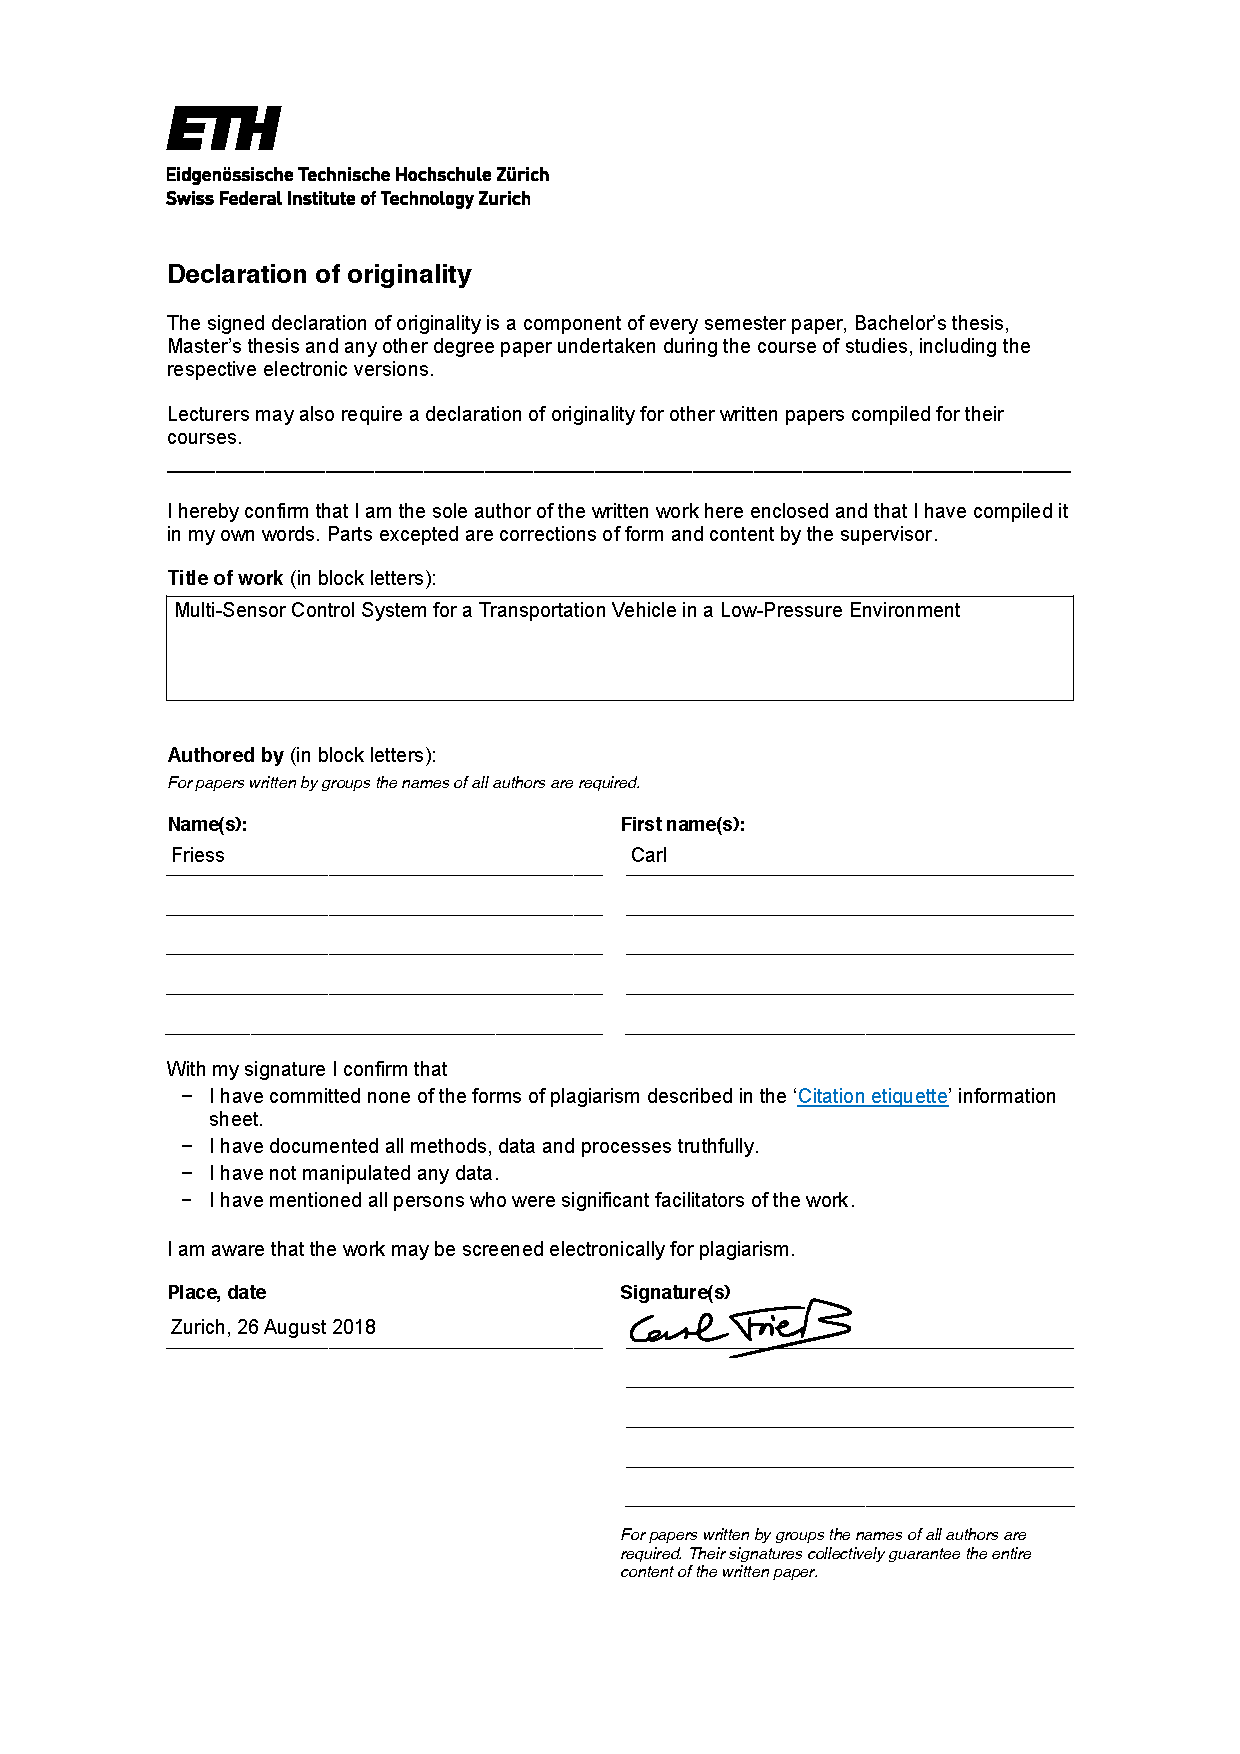
\includepdf[pages=-, turn=false, scale=0.9]{./figures/declaration_of_originality}


\backmatter

% Print the main glossary.
\printglossary[type=main,title=Glossary]


% Print the bibliography.
\nocite*{} % Print non-cited references as well.
\bibliographystyle{IEEEtran}
\bibliography{IEEEabrv,./bib/main}


\end{document}
%%%%%%%%%%%%%%%%%%%%%%%%%%%%%%%%%%%%%%%%%%%%%%%%%%%%%%%%%%%%%%%%%%%%%%%
%%%%%                                                                 %
%%%%%     End of Document                                             %
%%%%%                                                                 %
%%%%%%%%%%%%%%%%%%%%%%%%%%%%%%%%%%%%%%%%%%%%%%%%%%%%%%%%%%%%%%%%%%%%%%%
